
\hypertarget{cv:registrarPaso}{\section{Registrar Paso}} \label{sec:registrarPaso}

	Esta funcionalidad le permitirá registrar uno paso perteneciente a una trayectoria dentro del caso de uso que se esta operando.

		\subsection{Procedimiento}

			%Pasos de procedimiento
			\begin{enumerate}
	
			\item Oprima el botón \IURegistrar{} de la pantalla \ref{fig:GestionarPasos} ''Gestionar Pasos''.
			
			\item Se mostrará la pantalla \ref{fig:registrarPaso} ''Registrar Paso''.

			%Pantalla
			\begin{figure}[H]
				\begin{center}
					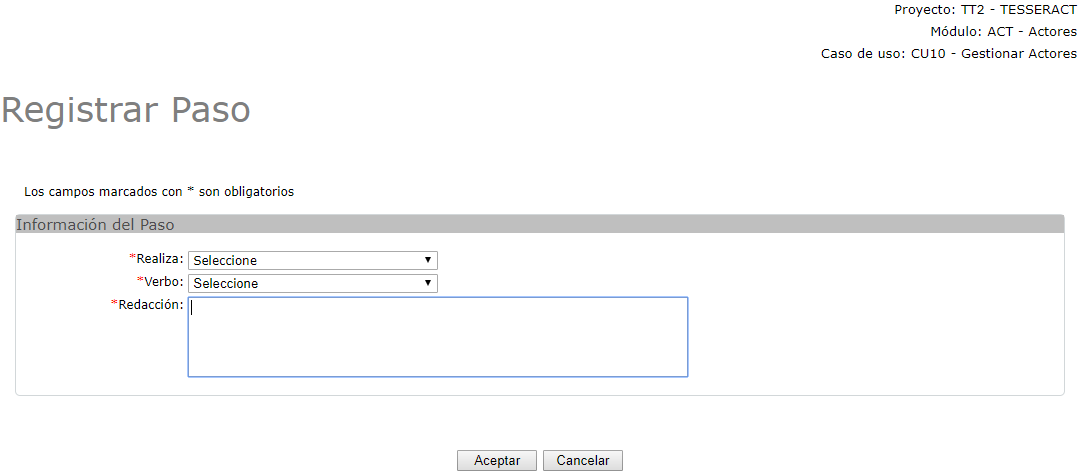
\includegraphics[scale=0.6]{roles/lider/casosUso/trayectorias/pasos/pantallas/IU6-1-1-1-1registrarPaso}
					\caption{Registrar Paso}
					\label{fig:registrarPaso}
				\end{center}
			\end{figure}
		
			\item Elija quien realiza el paso, el verbo con el que empieza e ingrese la redacción del paso.
			
			\item En la redacción usted podrá referenciar todos los tipos de elementos que se encuentren registrados dentro del proyecto actual, mendiante los siguientes TOKENS:
			
			\begin{itemize}
				\item Podrá referenciar elementos de tipo actor con el TOKEN: ''ACT·''.
				\item Podrá referenciar elementos de tipo entidad y/o atributos con los TOKEN: ''ENT·''y ''ATR·''.
				\item Podrá referenciar elementos de tipo regla de negocio con el TOKEN: ''RN·''.
				\item Podrá referenciar elementos de tipo caso de uso con el TOKEN: ''CU·''.
				\item Podrá referenciar elementos de tipo pantalla con el TOKEN: ''IU·''.
				\item Podrá referenciar elementos de tipo acción con el TOKEN: ''ACC·''.
				\item Podrá referenciar elementos de tipo mensaje con el TOKEN: 'MSG·''.
				\item Podrá referenciar elementos de tipo término con el TOKEN: ''GLS·''.
				\item Podrá referenciar elementos de tipo trayectoria con el TOKEN: ''TRAY·''.
				\item Podrá referenciar elementos de tipo paso con el TOKEN: ''P·''.
			\end{itemize}
			
			\item Oprima el botón \IUAceptar.
			
			\item Se mostrará el mensaje \ref{fig:pasoRegistrado} en la pantalla \ref{fig:GestionarPasos} ''Gestionar Pasos''.
			
			\begin{figure}[htbp!]
				\begin{center}
					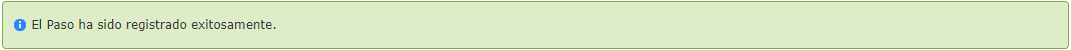
\includegraphics[scale=0.6]{roles/lider/casosUso/trayectorias/pasos/pantallas/IU6-1-1-1-1MSG1}
					\caption{MSG: Paso Registrado}
					\label{fig:pasoRegistrado}
				\end{center}
			\end{figure}
			\end{enumerate}